This chapter will evaluate Aparapi and JCuda - the two candidates who have got the highest marks - based on the test battery discussed in the previous chapter. At the end of this chapter, we will be able to compare the two solutions. This chapter will only be focusing on analyzing the solutions and the comparison between Aparapi and JCuda will come in the next chapter.

\section{Aparapi}

This section will evaluate Aparapi according to the test battery discussed in section \ref{battery test}.

Aparapi stands for A PAR\{allel\} API. It is a tool developed by AMD that gives the ability to write Java code for the GPU. Aparapi works with any configuration supporting a compatible OpenCL 1.1 runtime \cite{aparapiquestions}.

To be able to send GPU jobs, Aparapi dynamically translates Java bytecode at runtime to OpenCL instructions \cite{aparapiblog}. This makes the process of using Aparapi very transparent from the developer's point of view.

\subsection{Installation}

Using Aparapi only requires to include a library jar at the compilation stage and at the execution time. Once done, one can use the Aparapi's API to write specific GPU code.

The jar library comes with several examples that shows how to compile and write code. While we couldn't easily found a getting started guide, but we rapidly understood the process reading some examples.

Aparapi doesn't need any software installation except having a working OpenCL runtime. It only requires to include a jar in the compilation and execution stages and setting up the correct LD\_LIBRARY\_PATH containing the shared object (.so) library.

The following code shows a typical compilation and run process :

\begin{lstlisting}
$ javac -cp aparapi.jar:. GPLevenshtein.java
$ java -cp aparapi.jar:. GPLevenshtein 1000
\end{lstlisting}

The next listing shows how we included the shared object library:

\begin{lstlisting}
$ export LD_LIBRARY_PATH=$LD_LIBRARY_PATH:/path/to/foler
\end{lstlisting}

The process of using Aparapi is nearly the same as writing CPU threads \cite{aparapiarticle}. Basically, the kernel method will be in a class that inherits from Aparapi's Kernel class. The kernel method is called a given number of times when the class is instantiated. The following example uses Aparapi to perform the addition of two vectors:

\begin{lstlisting}
// The following class contains the kernel method that
// sums two vectors.
// The following code would runs the kernel :
// new AparapiLevenshtein(a,b,result).execute(a.length);
class AparapiExample extends Kernel {
  int[] a;
  int[] b;
  int[] result;
  
  public AparapiLevenshtein(int[] a, int[] b, int[] result) {
    this.a = a;
    this.b = b;
    this.result = result;
  }

  // Kernel method
  public void run() {
    int i = getGlobalId(); // The thread id
    result[i] = a[i] + b[i];
  }
}

\end{lstlisting}

\subsection{Matrix multiplication}

The code computing the matrix multiplication with Aparapi can be found in the appendix \ref{aparapi code}.

As seen in figure \ref{fig plot matrix aparapi}, aparapi gives a speedup up to 6 compared to a vanilla execution. It is interesting to note that the speedup is not constant over the matrix size (uncertainty may be the reason, see appendix \ref{uncertain}), but seems to stagnate around 5. The raw values of the speedup are available in the appendix \ref{raw values speedup aparapi matrix} and the uncertainty is discussed in appendix \ref{uncertain}.

\begin{figure}[H]
\centering
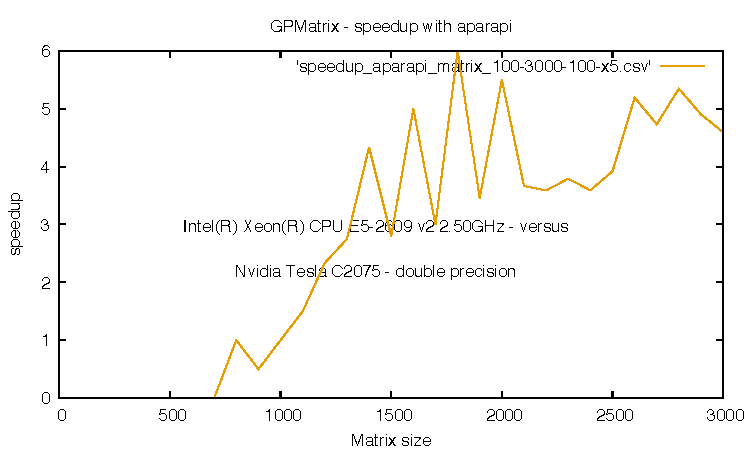
\includegraphics[width=1\textwidth]{speedup_aparapi_matrix_5x.pdf}
\caption{Speedup gained using Aparapi on matrix multiplication}
\label{fig plot matrix aparapi}
\end{figure}

Figure \ref{fig: plot aparapi matrix times} gives us sequential time running the matrix computation using vanilla Java and Aparapi. For each measure we took the average of 5 executions. We observe that using Aparapi on a GPU doesn't give a smooth curve. Those perturbations could be due to the operating system resource usages during the measures, but we didn't perform any other operations than executing the benchmark and repeated the measures 5 times. It is is probably due the rounding (see appendix \ref{uncertain}). The raw values of the sequential times using Aparapi on the matrix multiplication are available in the appendix \ref{raw values aparapi matrix}.

\begin{figure}[H]
\centering
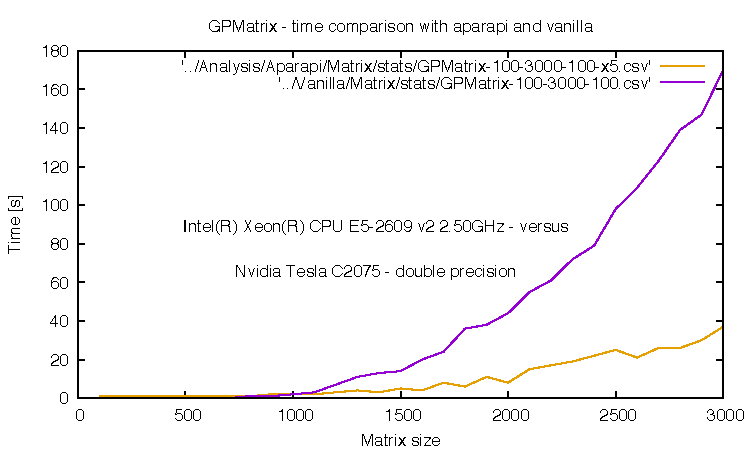
\includegraphics[width=1\textwidth]{time_aparapi_matrix_5x.pdf}
\caption{Times over matrix size using vanilla Java and Aparapi}
\label{fig: plot aparapi matrix times}
\end{figure}

Figure \ref{fig table matrix aparapi} gives some statistics about the speedup gained with our measures. Those metrics are specifics but, as will the others, it will give us the ability to compare them against another solution - like JCuda.

\begin{figure}[H]
\begin{center}
\begin{tabular}{ |l|l| } 
 \hline
 Speedup average & 2,3 \\ 
 Speedup median & 3.4 \\ 
 Speedup std. deviation & 1,8 \\ 
 \hline
\end{tabular}
\end{center}
\caption{Speedup statistics of matrix multiplication performed with Aparapi}
\label{fig table matrix aparapi}
\end{figure}

\subsection{Levenshtein distance}

The code computing the Levenshtein distance with Aparapi can be found in the appendix \ref{aparapi code}.

As seen in figure \ref{fig plot leven aparapi}, the speedup is at its best with a string size around 200'000 characters. Between this value, the speedup decreases. It is interesting to note that two different types of computation gives a significantly different speedup tendency. In this case, the algorithm is only really efficient around a specific string size range. The raw values of the speedup are available in the appendix \ref{raw values speedup aparapi Leven} and the uncertainty is discussed in appendix \ref{uncertain}.

\begin{figure}[H]
\centering
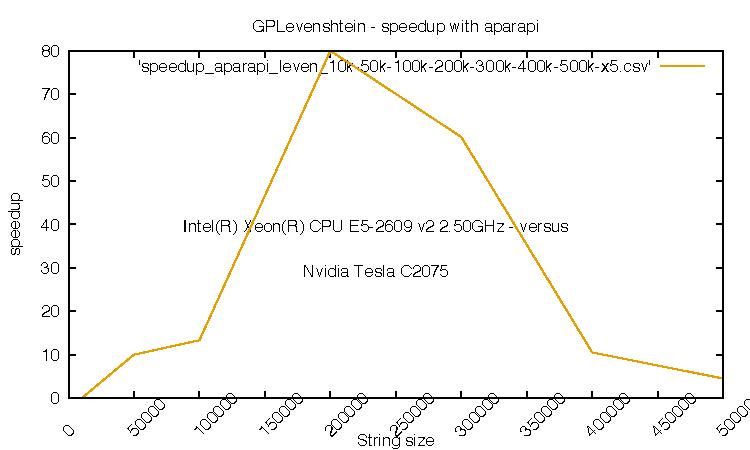
\includegraphics[width=1\textwidth]{speedup_aparapi_leven_5x.pdf}
\caption{Speedup gained using Aparapi on levenstein computation}
\label{fig plot leven aparapi}
\end{figure}

Figure \ref{fig: plot aparapi leven times} shows sequential time while running levenstein computation on a vanilla implementation and using Aparapi. We can observe that those curves have the same tendency and, around 200'000, show a small decreasing time for the Aparapi execution, thus giving the kind of 'mountain' for the speedup. Raw values of the sequential time using Aparapi for the Levenshtein distance computation is available in the appendix \ref{raw values aparapi leven}.

\begin{figure}[H]
\centering
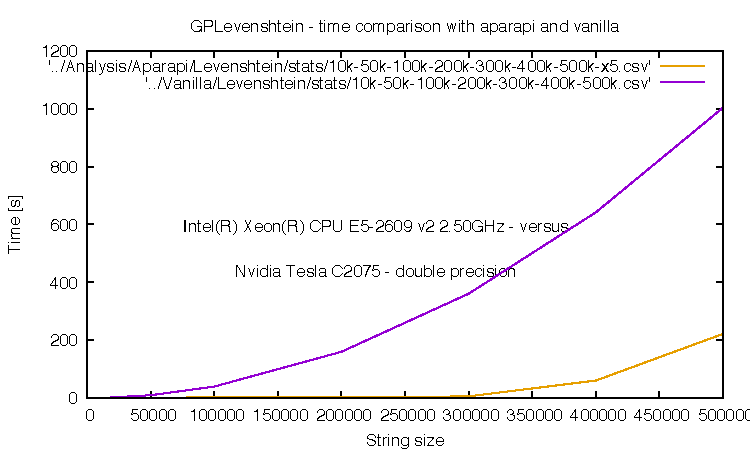
\includegraphics[width=1\textwidth]{time_aparapi_leven_5x.pdf}
\caption{Times over string sizes using java and Aparapi}
\label{fig: plot aparapi leven times}
\end{figure}

Figure \ref{fig table leven aparapi} shows some statistics of the speedup gained with our measures. As observed in figure \ref{fig plot leven aparapi}, we come with a high standard derivation, due to the kind of 'mountain' we obtained in our graph.

\begin{figure}[H]
\begin{center}
\begin{tabular}{ |l|l| } 
 \hline
 Speedup average & 25,2 \\ 
 Speedup median & 10 \\ 
 Speedup std. deviation & 29 \\ 
 \hline
\end{tabular}
\end{center}
\caption{Speedup statistics of levenstein computation performed with Aparapi}
\label{fig table leven aparapi}
\end{figure}

\subsection{External code feedback}

We asked 2 developers to evaluate the difficulty of using Aparapi to write GPU code. We gave them the Matrix multiplication and the Levenshtein distance source codes asking them to give a mark from 1 (very difficult to understand) to 5 (very easy to understand). The surveys can be found in the appendix \ref{aparapi code}.

Results are given in figure \ref{table aparapi code feedback}:

\begin{figure}[H]
\begin{center}
\begin{tabular}{ |l|l|l|l| } 
 \hline
  & \textbf{Matrix} & \textbf{Levenstein} \\
 \hline
 \textbf{Developper 1} & 5 & 5 \\ 
 \hline
 \textbf{Developper 2} & 5 & 5 \\ 
 \hline
\end{tabular}
\end{center}
\caption{Results of the Aparapi surveys. From 1 (very difficult to understand) to 5 (very easy to understand)}
\label{table aparapi code feedback}
\end{figure}

\subsection{LOC}

The number of code lines needed to use Aparapi for the matrix multiplication and Levenshtein distance computation are given in figure \ref{table aparapi loc}. Those numbers only include the methods used to compute the matrix multiplication and the Levenstein distance, removing comments and blank lines.

\begin{figure}[H]
\begin{center}
\begin{tabular}{ |l|l|l|l| } 
 \hline
 & \textbf{vanilla} & \textbf{Aparapi} & \textbf{delta} \\
 \hline
 \textbf{GPMatrix} & 13 & 21 & 8 \\ 
 \hline
 \textbf{GPLevenstein} & 18 & 24 & 6 \\ 
 \hline
\end{tabular}
\end{center}
\caption{LOC of GPMatrix and GPLevenstein using Aparapi compared to vanilla}
\label{table aparapi loc}
\end{figure}

\subsection{Overall feedback}

Installing and using Aparapi is quite straightforward. The first problem we met was to find an official documentation about installing and using Aparapi. While we couldn't find any relevant official documentation, we came up using a given example to take our first steps. Reading an example gave us enough information to start adapting our code using Aparapi.

The second problem we met was that using Java object inside the kernel function is not possible. We had to remove all Java object usages and adapt our implementation - for example by using a char array instead of a string in GPLevenstein. This restriction wasn't clearly documented by Aparapi.

The third problem we met was that getting the length of an array raised an error. After investigating, we found out that it is a know bug \cite{aparapibug}. This step took us a while to discover since the raised error wasn't explicit and didn't directly guide us to the real error's source.

In conclusion, Aparapi was quite easy to use despite the loss of an official and complete documentation. Not having the ability to use Java objects is disappointing and removes a major advantage of using Java code. But for specific uses, Aparapi is a simple and efficient solution to perform GPU computation inside Java code. 

\section{JCuda}

This section will evaluate JCuda according to the test battery discussed in section \ref{battery test}.

JCuda is a binding library that uses NVIDIA CUDA technologies. CUDA® is a parallel computing platform and programming model invented by NVIDIA. It enables dramatic increases in computing performance by harnessing the power of the graphics processing unit (GPU)\cite{cudahome}.

JCuda provides binding from Java to CUDA. The library enables programmers to write Java methods. Thoses methods will be automatically bound to the corresponding CUDA ones, which would be written in CUDAC/C++ \cite{cudagpgpu}.

With JCuda, programmers will have to write the kernel method in a separate native CUDA file (.cu) and use the JCuda library from Java to call the kernel and perform data transfers. The process is nearly similar as one would do with plain CUDA language, but using adapted Java methods.

\subsection{Installation}

The installation of JCuda requires the same process as with Aparapi. A jar library needs to be included in the compilation and execution stages and a library (shared object file on Linux) must be visible to Java at runtime (typically using LC\_LIBRARY\_PATH).

No extra software is needed, but only having a working CUDA environment setup and including the JCuda library.

The installation process is well documented as well as the first steps to write a first program using JCuda. There are also plenty of examples to help understanding how JCuda works.

A typical compilation and run case for a JCuda program would be something like :
\begin{lstlisting}
$ javac -cp ".:jcuda-0.7.5.jar" GPMatrix.java
$ java  -cp ".:jcuda-0.7.5.jar" GPMatrix 1000
\end{lstlisting}

To get an idea of how JCuda works, the following listing shows an example of a two vectors addition using JCuda :

\begin{lstlisting}
// From the Java class
  ...
  int[] A = ...; int[] B = ...;
  int[] result = ...; int size = a.length;
  
  // Create the PTX file by calling the NVCC
  String ptxFileName = preparePtxFile("kernel.ptx");
  
  // Load the CUDA kernel ptx file
  CUmodule module = new CUmodule();
  cuModuleLoad(module, ptxFileName);

  // Obtain a function pointer to the kernel function
  CUfunction function = new CUfunction();
  cuModuleGetFunction(function, module, "add");

  // Allocate the device input/output data, and 
  // copy the host input data to the device
  int ptrSize = size * Sizeof.INT;
  CUdeviceptr deviceInputA = new CUdeviceptr();
  cuMemAlloc(deviceInputA, ptrSize);
  cuMemcpyHtoD(deviceInputA, Pointer.to(A), ptrSize);

  CUdeviceptr deviceInputB = new CUdeviceptr();
  cuMemAlloc(deviceInputB, ptrSize);
  cuMemcpyHtoD(deviceInputB, Pointer.to(B), ptrSize);

  CUdeviceptr deviceOutput = new CUdeviceptr();
  cuMemAlloc(deviceOutput, ptrSize);

  // Set up the kernel parameters: A pointer to an array
  // of pointers which points to the actual values
  Pointer kernelParameters = Pointer.to(
    Pointer.to(deviceInputA),
    Pointer.to(deviceInputB),
    Pointer.to(deviceOutput),
    Pointer.to(new int[]{size})
  );

  // Kernel call parameters
  int blockSizeX = 256;
  int gridSizeX = (int)Math.ceil((double)size / blockSizeX);

  // --------------------------------
  long startTime = System.currentTimeMillis();
  // --- Start of benchmark zone --->
  cuLaunchKernel(function,
    gridSizeX, 1, 1,       // Grid dimension
    blockSizeX, 1, 1,     // Block dimension
    0, null,              // Shared memory size and stream
    kernelParameters, null // Kernel and extra parameters
  );
  cuCtxSynchronize();
  
  // Get the result
  cuMemcpyDtoH(Pointer.to(result), deviceOutput, ptrSize);
...

// Kernel.cu
extern "C"
__global__ void add(int* A, int* B, int* result, int size) {
  int i = blockIdx.x * blockDim.x + threadIdx.x;

  if(i < size) {
    result[i] = A[i] + A[i];
  }
}

\end{lstlisting}

\subsection{Matrix multiplication}

Like we did with Aparapi, we took the matrix multiplication vanilla code and ported the same portion of code as with Aparapi to the GPU. We then made the same measures as with Aparapi and computed the speedup gained between JCuda and vanilla Java code. The adapted code can be found in the appendix \ref{jcuda code}.

Figure \ref{fig plot matrix jcuda} shows the speedup gained using JCuda in the matrix multiplication code. We can see that we obtained a speedup rising up to 12. The shape of the curve is not constantly rising, but is giving a maximum around a matrix size between 2000 and 2500.

So as to prevent edge cases and removing noise, we each time took 5 measures and used the average values between the 5 results. Raw values for the speedup using JCuda on the matrix multiplication are available in the appendix \ref{raw values speedup jcuda matrix} and the uncertainty is discussed in appendix \ref{uncertain}.

\begin{figure}[H]
\centering
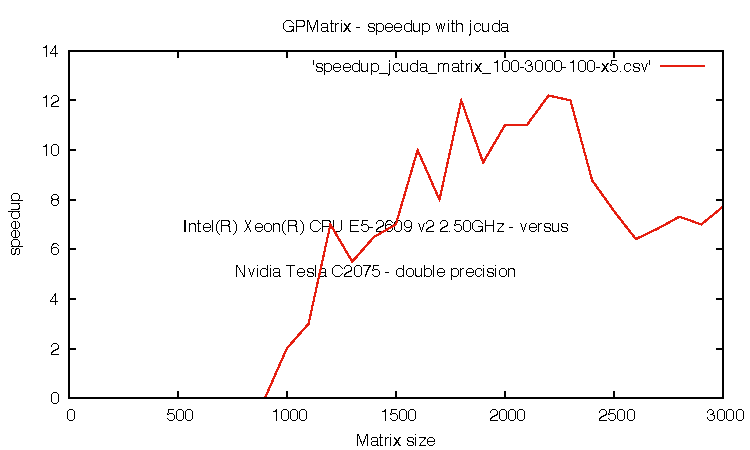
\includegraphics[width=1\textwidth]{speedup_jcuda_matrix_5x.pdf}
\caption{Speedup gained using JCuda on matrix multiplication}
\label{fig plot matrix jcuda}
\end{figure}

Figure \ref{fig: plot jcuda matrix times} gives us sequential times of the vanilla execution and the JCuda one on the matrix multiplication. The sequential times with JCuda seem to expand on a logarithm form while the sequential times on the vanilla code expand more in an exponential manner. Raw values of the sequential times using JCuda on the matrix multiplication can be found in the appendix \ref{raw values jcuda matrix}.

\begin{figure}[H]
\centering
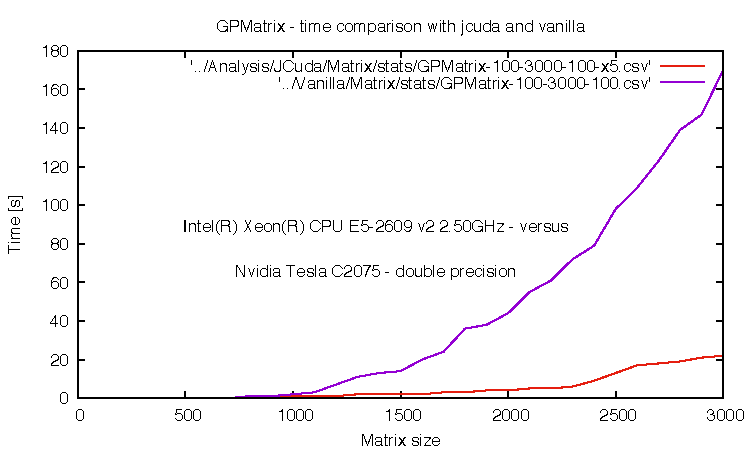
\includegraphics[width=1\textwidth]{time_jcuda_matrix_5x.pdf}
\caption{Times over matrix size using Java and JCuda}
\label{fig: plot jcuda matrix times}
\end{figure}

Figure \ref{fig table matrix jcuda} are some statistics on the speedup gained using JCuda. Those values will later be used to have metrics to compare between JCuda and Aparapi.

\begin{figure}[H]
\begin{center}
\begin{tabular}{ |l|l| } 
 \hline
 Speedup average & 5.6 \\ 
 Speedup median & 7 \\ 
 Speedup std. deviation & 4.3 \\ 
 \hline
\end{tabular}
\end{center}
\caption{Speedup statistics of matrix multiplication performed with JCuda}
\label{fig table matrix jcuda}
\end{figure}

\subsection{Levenshtein distance}

Figure \ref{fig plot leven jcuda} is the speedup gained using JCuda for the Levenshtein distance against vanilla code. The speedup gives its highest peak around a string size of 200'000 and decreases after. We observed the same behavior using Aparapi. Measures were based on an average of 5 executions and raw values are available in appendix \ref{raw values speedup jcuda Leven}. The uncertainty is discussed in appendix \ref{uncertain}. Full code can also be found in the appendix \ref{jcuda code}.

Unlike with the matrix multiplication, Aparapi gave a better peak with a speedup of nearly 80, while JCuda is around 55 at its highest peak.

\begin{figure}[H]
\centering
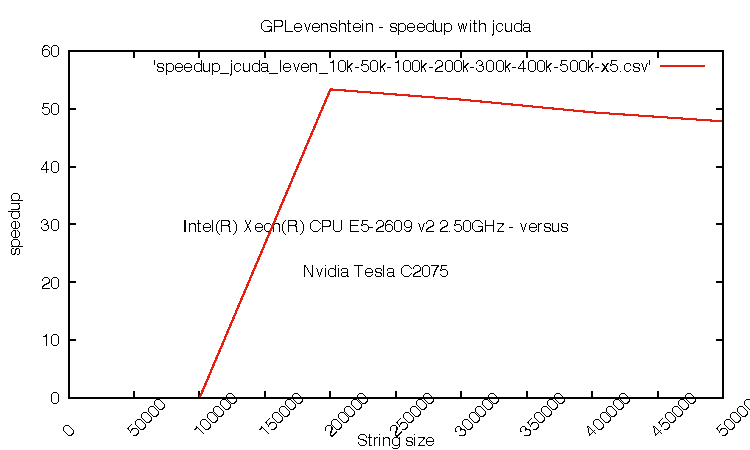
\includegraphics[width=1\textwidth]{speedup_jcuda_leven_5x.pdf}
\caption{Speedup gained using JCuda on Levenstein distance computation}
\label{fig plot leven jcuda}
\end{figure}

Figure \ref{fig: plot jcuda leven times} shows sequential times while executing the Levenshtein distance computation on different string sizes with JCuda and  vanilla Java, this on the same graph. Sequential times for JCuda are ridiculously small compared to the vanilla Java. Those measures are based on an average of 5 executions. Raw values of the execution times for the Levenstein distance computation using JCuda are available in appendix \ref{raw values jcuda leven}.

Statistics about the speedup are available in figure \ref{fig table leven jcuda}.

\begin{figure}[H]
\centering
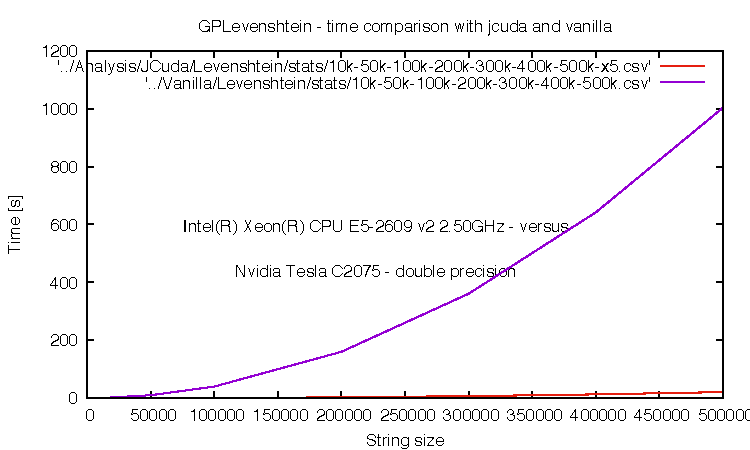
\includegraphics[width=1\textwidth]{time_jcuda_leven_5x.pdf}
\caption{Times over string size using Java and JCuda}
\label{fig: plot jcuda leven times}
\end{figure}

\begin{figure}[H]
\begin{center}
\begin{tabular}{ |l|l| } 
 \hline
 Speedup average & 28.5 \\ 
 Speedup median & 47.8 \\ 
 Speedup std. deviation & 24.8 \\ 
 \hline
\end{tabular}
\end{center}
\caption{Speedup statistics of Levenstein computation performed with JCuda}
\label{fig table leven jcuda}
\end{figure}

\subsection{External feedback}

We asked 2 developers to evaluate the difficulty of using JCuda to write GPU code. We gave them the Matrix multiplication and the Levenshtein distance source codes, asking them to give a mark from 1 (very difficult to understand) to 5 (very easy to understand). The surveys can be found in the appendix \ref{jcuda code}.

Results are given in the figure \ref{table jcuda code feedback}:

\begin{figure}[H]
\begin{center}
\begin{tabular}{ |l|l|l|l| } 
 \hline
  & \textbf{Matrix} & \textbf{Levenstein} \\
 \hline
 \textbf{Developper 1} & 4 & 3 \\ 
 \hline
 \textbf{Developper 2} & 4 & 3 \\ 
 \hline
\end{tabular}
\end{center}
\caption{Results of the JCuda surveys. From 1 (very difficult to understand) to 5 (very easy to understand)}
\label{table jcuda code feedback}
\end{figure}

\subsection{LOC}

The numbers of code lines needed to use JCuda for the matrix multiplication and Levenshtein distance computation are given in figure \ref{table jcuda loc}. Those numbers include only the methods used to compute the matrix multiplication and the Levenshtein distance, removing comments and blank lines.

\begin{figure}[H]
\begin{center}
\begin{tabular}{ |l|l|l|l| } 
 \hline
 & \textbf{vanilla} & \textbf{JCuda} & \textbf{delta} \\
 \hline
 \textbf{GPMatrix} & 13 & 47 & 30 \\ 
 \hline
 \textbf{GPLevenstein} & 18 & 51c & 25 \\ 
 \hline
\end{tabular}
\end{center}
\caption{LOC of GPMatrix and GPLevenstein using JCuda compared with vanilla}
\label{table jcuda loc}
\end{figure}

\subsection{Overall feedback}

JCuda is really well documented and easy to install. Due to its binding philosophy, using JCuda gives more the impression of writing CUDA code in Java than using Java to write GPU code. The fact that the kernel method is written in C is the main reason, but also the way we allocate and set the kernel's parameters. From Java, all we do is calling the kernel exactly as we would with CUDA, but with Java methods. This can be disturbing for someone who has no experience using CUDA, but on the other hand, if someone has already a CUDA experience, it won't be difficult at all to get started.

A major restriction of using JCuda is due to the kernel written in C. It does not allow developers to use Java code and breaks the process of a pure Java development workflow. This lets only the possibility to write a single c method. In our case, for example, we couldn't use or write a simple method \textbf{min()} that would make the code much easier to read in our kernel. But, in the other hand, an advantage of using the kernel in its pure form, written in C, is the fact that it makes possible to use already written CUDA kernel methods. Hence making the process of kernel reusability among other existing projects possible. This aspect should be worth considering in some context.

In conclusion, JCuda was easy to install, well documented and relatively fast to get started with. Using pure kernel methods in C could be interesting for someone familiar with CUDA, but does not have the advantage of using Java code. For Java code that needs to execute specific instructions to the GPU on a CUDA architecture, JCuda is a good solution as long as the kernel does not need any Java objects and/or methods.